\documentclass[letterpaper, 12pt]{article}

\usepackage{geometry}
 \geometry{
 letterpaper,
 total={170mm,257mm},
 left=20mm,
 top=20mm,
 bottom=20mm
 }
\usepackage{graphicx} % Required for inserting images
\usepackage{authblk}
\usepackage{amssymb}
\usepackage{lipsum}
\usepackage{float}
\usepackage{times}
\usepackage{amsmath}
\usepackage[format=plain,
            labelfont={bf,it},
            textfont=it]{caption}
\captionsetup{justification=raggedright,singlelinecheck=false}
\usepackage{ragged2e}
\usepackage{longtable}
\usepackage{comment}
\usepackage{setspace}
\usepackage{fancyhdr}
\usepackage{titlesec}
\usepackage[hyperindex,breaklinks]{hyperref}
\hypersetup{
    colorlinks=true,
    linkcolor=blue,
    filecolor=magenta,      
    urlcolor=blue,
    pdftitle={Overleaf Example},
    pdfpagemode=FullScreen,
    }
% \usepackage{background} % add COSIG logo to page
\usepackage[T1]{fontenc}
\usepackage{helvet}
\renewcommand{\familydefault}{\sfdefault}
\pagenumbering{gobble}
\usepackage[skip=10pt plus1pt, indent=40pt]{parskip}

\titlespacing*{\section}
{0pt}{1.5ex plus 1ex minus .2ex}{1.3ex plus .2ex}

\renewcommand\Authfont{\fontsize{12}{14.4}\selectfont}
\renewcommand\Affilfont{\fontsize{9}{10.8}\itshape}
 
\begin{document}
\flushleft

\includegraphics[width=0.5\textwidth]{img/home/241017_final_logo_mockup.png}

\section*{Image duplication}
\addcontentsline{toc}{section}{Image duplication}
\textit{Last updated: 17 April 2025}

Image duplication is one of the most frequently spotted integrity issues in scientific publications. This term is generally used to describe instances where two images (or parts of an image) are supposed to represent different things but are actually identical.

\href{https://doi.org/10.1128/mbio.00809-16}{Bik et al. (2016)} established a typology of image duplications, summarized below. Additional examples are provided in the external resources listed at the end of this guide.

\subsection*{Type I: Simple duplication}

This describes when the same image has been used multiple times in an article to represent different experiments or samples. Sometimes, the same image is used multiple times in an article to represent the same experiment, which is usually not considered problematic.

\subsection*{Type II: Duplication with repositioning}

This describes when the same image has been used multiple times in an article to represent different experiments or samples, but in one or more of these instances the image has been cropped, rotated, flipped or otherwise repositioned.

\subsection*{Type III: Duplication with alteration} 

This describes when the same image has been used multiple times in an article to represent different experiments or samples, but one or more instances of this image have been altered relative to the others via the addition or subtraction of certain features. This category also covers duplicated regions within a single image shown in 
an article.

Among the above categories, Type I is considered the least severe (and most likely to be the result of an error during figure preparation) while Type III is considered the most severe (and most likely to be the result of deliberate image manipulation). 

As noted by \href{https://doi.org/10.1017/jme.2025.32}{Brookes (2025)}, images can also be duplicated between different articles. In these cases, it is problematic when these images are supposed to represent different experiments or have not been properly attributed to the original authors that collected or published the image.

\subsection*{Common false positives}

Review articles will often republish images used in previous articles. This is only problematic if the review article misrepresents the image being used or does not properly attribute it to its original source.

Many articles will include images from publicly-available datasets (e.g., the \href{https://www.cs.toronto.edu/~kriz/cifar.html}{CIFAR datasets} or histopathology images from the \href{https://www.proteinatlas.org/}{Human Protein Atlas}). Again, as long as these images are properly attributed and not misrepresented, this is not problematic.

The different channels in \href{https://en.wikipedia.org/wiki/Fluorescence_microscope}{fluorescence microscopy} images are often displayed in separate panels alongside a panel where all channels are merged. Although it may appear that these images are inappropriately duplicated, they in fact represent the same data and presenting images in this way is not problematic.

\subsection*{Annotating image duplications}

When reporting observations of image duplications on PubPeer or to journal editors, it is often useful to illustrate exactly which images / regions are apparently duplicated. This is often accomplished by overlaying colored boxes on the image (as shown in the examples below) where each color corresponds to a different set of shared image features. These annotations are usually performed in software like \href{https://www.microsoft.com/en-us/windows/paint}{Microsoft Paint}, \href{https://www.gimp.org/}{GIMP} or \href{https://www.microsoft.com/en-us/microsoft-365/powerpoint}{Microsoft PowerPoint}. 

If annotating an article with many apparent duplications, you may find yourself running out of unique colors to use. Using too many colors can make annotations difficult to interpret. Strive for readability when annotating images -- it is often useful to show the original image alongside the annotated image.

\begin{figure}[h!tbp]
    \centering
    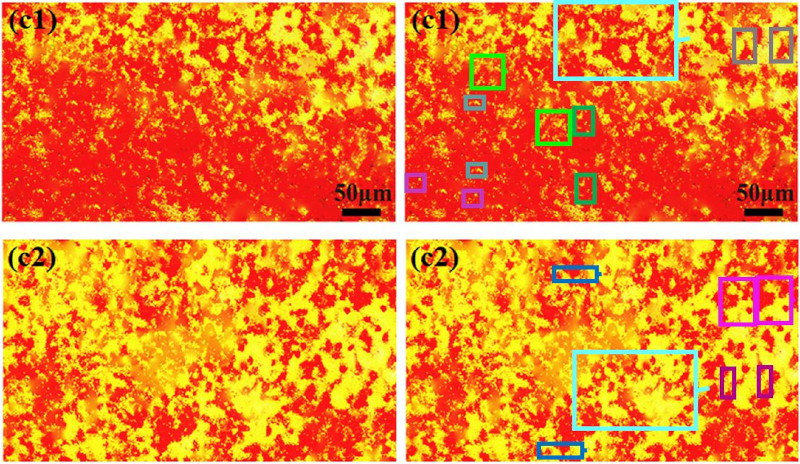
\includegraphics[width=0.8\textwidth]{img/image_duplication/Bakhsheshi-Rad_annotation.JPG}
    \caption*{An original set of published images of cell culture (left) versus an annotated version of these images showing regions of unusually high similarity (right). Adapted from Figure 4C of \href{https://doi.org/10.1016/j.polymertesting.2019.106298}{Bakhsheshi-Rad et al. (2020)}.}
\end{figure}

For Type II and Type III duplications that involve rotation or flipping, it is often useful to attach a small symbol to each of the boxes to make it more apparent what transformation occurred, such as a small diagonal line on the side of the box. 

A PowerPoint template containing several pre-made boxes and symbols for annotating images is \href{https://osf.io/w3epj}{available here}.

\subsection*{Example 1: Type I duplication}

\href{https://doi.org/10.1172/JCI66764}{Morrison et al. (2013)} describe experiments in breast cancer cell cultures with visible light microscopy images. However, two of the images used in Figure 4 to describe different experimental conditions are identical.

\begin{figure}[h!tbp]
    \centering
    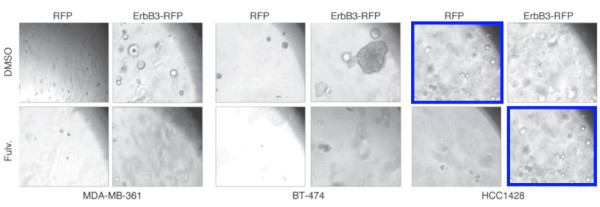
\includegraphics[width=\textwidth]{img/image_duplication/image-1744937326665.jpg}
    \caption*{Two panels representing different experimental conditions (one representing RFP-expressing cells treated with DMSO and one representing ErbB3-RFP-expressing cells treated with fulvestrant) are identical, as indicated by blue boxes. Adapted from Figure 4 of \href{https://doi.org/10.1172/JCI66764}{Morrison et al. (2013)} by \href{https://pubpeer.com/publications/2768B5B42E7338AB72D4CFE660596A\#1}{Sholto David on PubPeer}.}
\end{figure}

\pagebreak

\subsection*{Example 2: Type II duplication}

Morrison et al. also provide histopathological images of implanted tumors. One image shown in Figure 2 and one image shown in Figure 7 show the same sample despite representing different treatments. The image shown in Figure 2 is cropped differently than that shown in Figure 7.

\begin{figure}[h!tbp]
    \centering
    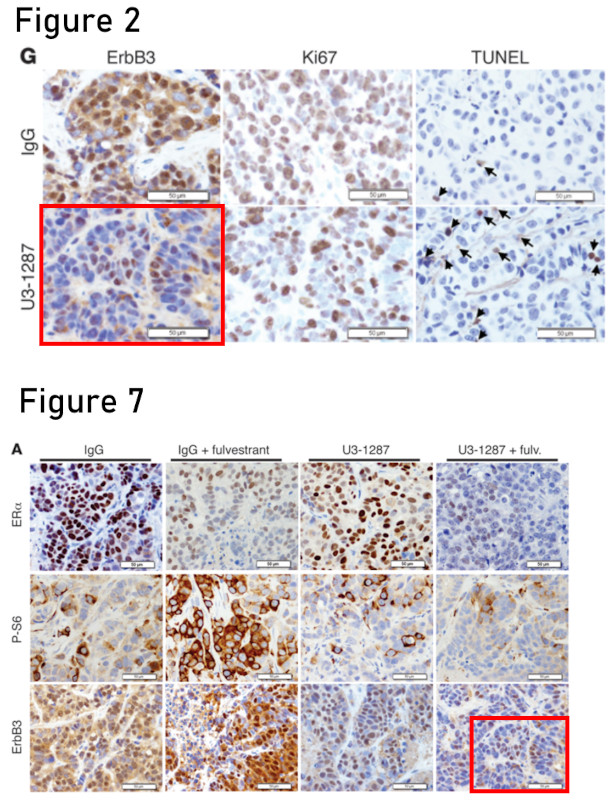
\includegraphics[width=0.7\textwidth]{img/image_duplication/image-1744937642757.jpg}
    \caption*{Two panels representing different experimental conditions (one representing tumor-bearing mice treated with antibody U3-1287 and one representing tumor-bearing mice treated with antibody U3-1287 and fulvestrant) show the same sample. The two images are cropped differently. The region the two images share in common is highlighted with red boxes. Adapted from \href{https://doi.org/10.1172/JCI66764}{Morrison et al. (2013)} by \href{https://pubpeer.com/publications/2768B5B42E7338AB72D4CFE660596A\#2}{Sholto David on PubPeer}.}
\end{figure}

\subsection*{Example 3: Type III duplication}

\href{https://doi.org/10.1007/s10853-015-9003-3}{Mohaghegh et al. (2015)} report synthesizing crystal nanoparticles. One of the scanning electron microscope (SEM) images they show of their synthesized particles contain regions that are exactly identical to one another. This is very unlikely to have occured by chance.

\begin{figure}[h!tbp]
    \centering
    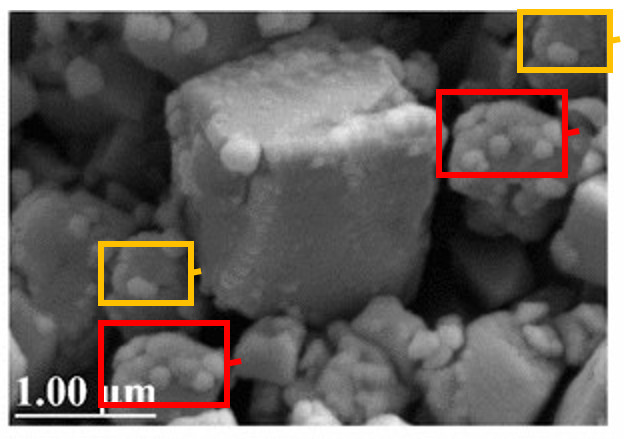
\includegraphics[width=\textwidth]{img/image_duplication/image-1741643734642.jpg}
    \caption*{In this SEM image of nanoparticles, the colored boxes shown here enclose regions that are exactly identical to one another. Adapted from Figure 3A of \href{https://doi.org/10.1007/s10853-015-9003-3}{Mohaghegh et al. (2015)} by \href{https://pubpeer.com/publications/7BE7C2A93C385F700F1C6B5BC90294\#1}{Reese Richardson on PubPeer}.}
\end{figure}

\pagebreak

\subsection*{Example 4: Type II duplication between articles}

\href{https://doi.org/10.3390/ph16070925}{Badr et al. (2023)} reuses a scanning electron microscope image previously used by \href{https://doi.org/10.2147/ijn.s77731}{Kurakala et al. (2015)} to represent a different material. In Badr et al., the image has been rotated 180 degrees and cropped. The metadata banners included in the image are inconsistent with one another and show wildly different scale bars. Because the metadata banners appear to have been altered, this could also be classified as a Type III duplication.

\begin{figure}[h!tbp]
    \centering
    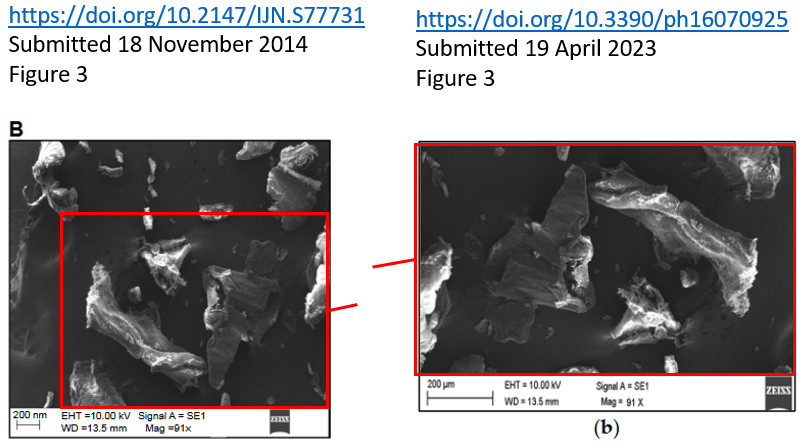
\includegraphics[width=\textwidth]{img/image_duplication/image-1741998932949.jpg}
    \caption*{\href{https://doi.org/10.3390/ph16070925}{Badr et al. (2023)} uses a scanning electron microscope image to represent itopride hydrochloride. The same image was previously used by \href{https://doi.org/10.2147/ijn.s77731}{Kurakala et al. (2015)} to represent chitosan. Note that the two images are accompanied by inconsistent scale bars (the scale bar in the Kurakala et al. image suggests particles one thousand times larger than that shown by Badr et al.). The image shown by Badr et al. has been cropped and rotated 180 degrees relative to the image shown by Kurakala et al. The shared region is shown with red boxes (note that a small diagonal line is affixed to each of these boxes to make their relative rotation more apparent). Adapted from Badr et al. and Kurakala et al. by \href{https://pubpeer.com/publications/30DDCFCF4925C0DD401AA9810AC0A3}{Reese Richardson on PubPeer}.}
\end{figure}

\pagebreak

\subsection*{Example 5: Type III duplication}

\href{https://doi.org/10.1371/journal.pone.0058855}{Zhou et al. (2013)} report on protein expression in one experiment using Western blots. In one of their Western blots, two of the lanes shown representing particular time points appear identical to the adjacent two lanes representing later time points. This article was \href{https://doi.org/10.1371/journal.pone.0322907}{retracted in 2025} for image integrity concerns and use of \href{https://osf.io/d7we5}{contaminated cell lines}.

\begin{figure}[h!tbp]
    \centering
    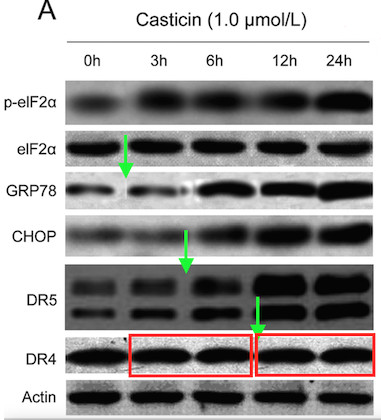
\includegraphics[width=0.7\textwidth]{img/image_duplication/image-1583362705327.jpg}
    \caption*{The 3h and 6h lanes of the DR4 panel of this series of Western blot images are identical to the 12h and 24h lanes, as shown with red boxes. Vertical green arrows indicate sharp vertical transitions between lanes, representing potential instances where images have been spliced. Adapted from Figure 6A of \href{https://doi.org/10.1371/journal.pone.0058855}{Zhou et al. (2013)} by \href{https://pubpeer.com/publications/2596C5A7287C83AFB4518CEF8AF7B4\#1}{Elisabeth Bik on PubPeer}.}
\end{figure}

\pagebreak

\subsection*{Example 6: False positive, merged fluorescence microscopy image, no image duplication}

\href{https://doi.org/10.1371/journal.pone.0083018}{Lepore et al. (2013)} use fluorescence microscopy to visualize protein localization within individual cells. As is conventional for this type of data, they represent their fluorescence microscopy images as separate images for each channel (green and blue) as well as an image that merges both channels. The merged image appears similar to the images with separated channels because it represents the exact same data. Thus, there is no problematic image duplication here.

\begin{figure}[h!tbp]
    \centering
    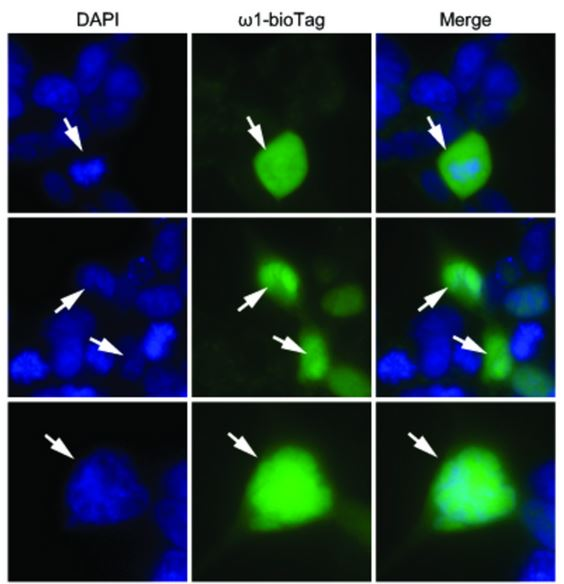
\includegraphics[width=0.7\textwidth]{img/image_duplication/merge.JPG}
    \caption*{Fluorescence microscopy images where each row contains an image showing the DAPI (blue, left) channel, the $\omega$1-bioTag (green, center) channel and a merged channel (right). Adapted from Figure 6D of \href{https://doi.org/10.1371/journal.pone.0083018}{Lepore et al. (2013)}.}
\end{figure}


\subsection*{Additional resources}

\begin{itemize}
    \setlength\itemsep{-0.5em}
    \item \href{https://doi.org/10.1128/mbio.00809-16}{``The Prevalence of Inappropriate Image Duplication in Biomedical Research Publications'' (2016)}
    \item \href{https://scienceintegritydigest.com/2020/01/08/types-of-image-duplications/}{``Types of image duplications: the palm trees'' (2020)}
    \item \href{https://doi.org/10.1017/jme.2025.32}{``Misconduct Detection — Evolving Methods \& Lessons from 15 Years of Scientific Image Sleuthing'' (2025)}
    \item \href{https://osf.io/g23pf}{COSIG: Software for image forensics}
\end{itemize}

\end{document}